\fancyhead[R]{Python Application Energy Consumption}
\section{Results}
\label{sec:results}

Each recording made with the Otii software samples power draw in watts 10,000 times per second. For every unique configuration of RPi, OS, and Python version, 10 recordings are made -- one for each benchmarking run. Average power draw and the runtime in seconds are extracted from each individual recording, with energy consumption in joules being calculated immediately as well. These results are then written to a CSV file uniquely named by the three parameters, e.g. \texttt{results\_RPi3B+\_Alpine\_python3.9.csv}, such that every CSV file contains the results for the 10 recordings made for that configuration. The CSV files can all be found in the repository.  

\begin{figure}[H]
    \centering
    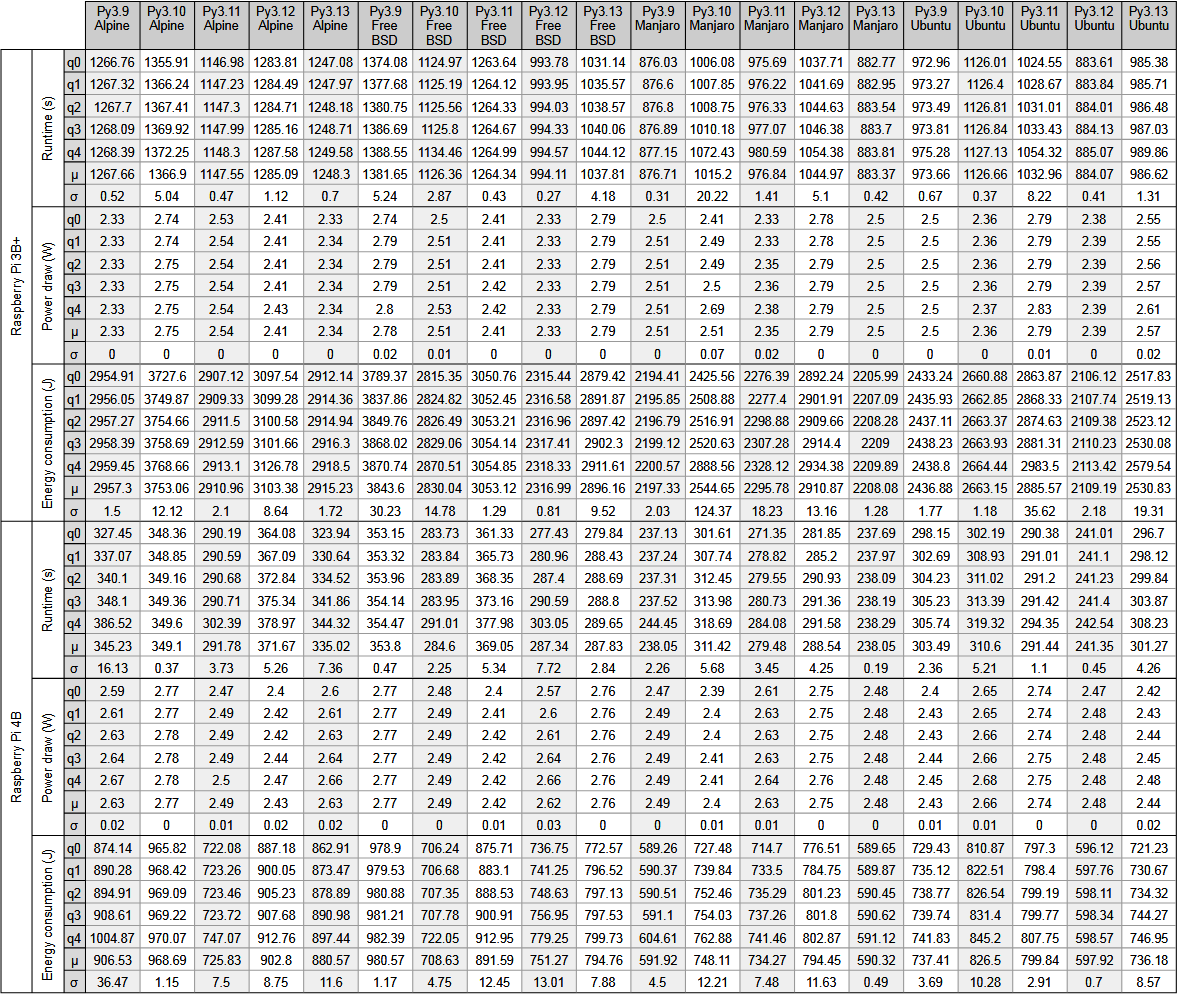
\includegraphics[width=1\textwidth]{figures/summary_stats_all.PNG}
    \caption{Table showing descriptive statistics for the energy consumption, power draw and runtime for each of the 40 configurations tested.}
    \label{fig:statstable}
\end{figure}

\autoref{fig:statstable} presents a comprehensive summary of descriptive statistics for all benchmark runs, grouped by Raspberry Pi model, Python version, and operating system. For each configuration, the table includes key metrics: runtime (in seconds), power draw (in watts), and derived energy consumption (in joules). To capture the distribution and variability of these measurements, each metric is summarised thusly: $q_0$ denotes the minimum, $q_1$ the 25th quartile, $q_2$ the median, $q_3$ the 75th quartile, $q_4$ the maximum, $\mu$ is the arithmetic mean, or average, and the standard deviation is denoted by $\sigma$. These seven values are presented for every unique configuration, meaning they are computed from the 10 recordings made for that configuration, as mentioned above. The significance of the values can be understood as follows: The median ($q_2$) provides a measure of central tendency, which is valuable when distributions are skewed or contain outliers. The mean ($\mu$) reflects the average, which is sensitive to extreme values and therefore helps understand the general tendencies in that configuration. The quartiles ($q_1$ and $q_3$) indicate the spread of the central 50\% of the data, allowing assessment of variability within the runs. The minimum ($q_0$) and maximum ($q_4$) values help understand the full range of recorded values, highlighting potential outliers or unstable configurations. Finally, the standard deviation ($\sigma$) quantifies the dispersion around the mean. Low $\sigma$ values suggest consistent performance across repeated runs, whereas higher $\sigma$ indicates variability, which makes the results less reliable. With this in mind, one of the first observations to be made is the low standard deviation seen across all configurations, which is promising for the reliability of the results. Comparing configurations, the longest average duration was for RPi3B+ on FreeBSD running Python3.10 ($q_0$: $\sim$1374s, $q_1$: $\sim$1377s, $q_2$: $\sim$1380s, $q_3$: $\sim$1386s, $q_4$: $\sim$1388.5s, $\mu$: $\sim$1381s, $\sigma$: $\sim$5.2s), while the shortest was for RPi4B on Manjaro running Python3.11 ($q_0$: $\sim$237s, $q_1$: $\sim$237s, $q_2$: $\sim$237s, $q_3$: $\sim$237s, $q_4$: $\sim$244.4s, $\mu$: $\sim$238s, $\sigma$: $\sim$2.3s). The highest average power draw was for RPi3B+ on FreeBSD running Python3.13 ($q_0$: $\sim$2.8W, $q_1$: $\sim$2.8W, $q_2$: $\sim$2.8W, $q_3$: $\sim$2.8W, $q_4$: $\sim$2.8W, $\mu$: $\sim$2.8W, $\sigma$: $\sim$0.01W), with the lowest being RPi3B+ on Alpine running Python3.11 ($q_0$: $\sim$2.3W, $q_1$: $\sim$2.3W, $q_2$: $\sim$2.3W, $q_3$: $\sim$2.3W, $q_4$: $\sim$2.3W, $\mu$: $\sim$2.3W, $\sigma$: $\sim$0.00W).
Finally, looking at energy consumption, the highest was RPi3B+ on FreeBSD running Python3.10 ($q_0$: $\sim$3789J, $q_1$: $\sim$3837J, $q_2$: $\sim$3849J, $q_3$: $\sim$3868J, $q_4$: $\sim$3870J, $\mu$: $\sim$3843J, $\sigma$: $\sim$30J) and the lowest was for RPi4B on Manjaro running Python3.12
($q_0$: $\sim$589J, $q_1$: $\sim$589J, $q_2$: $\sim$590J, $q_3$: $\sim$590J, $q_4$: $\sim$591J, $\mu$: $\sim$590J, $\sigma$: $\sim$0.5J).  

\begin{figure}[H]
    \centering
    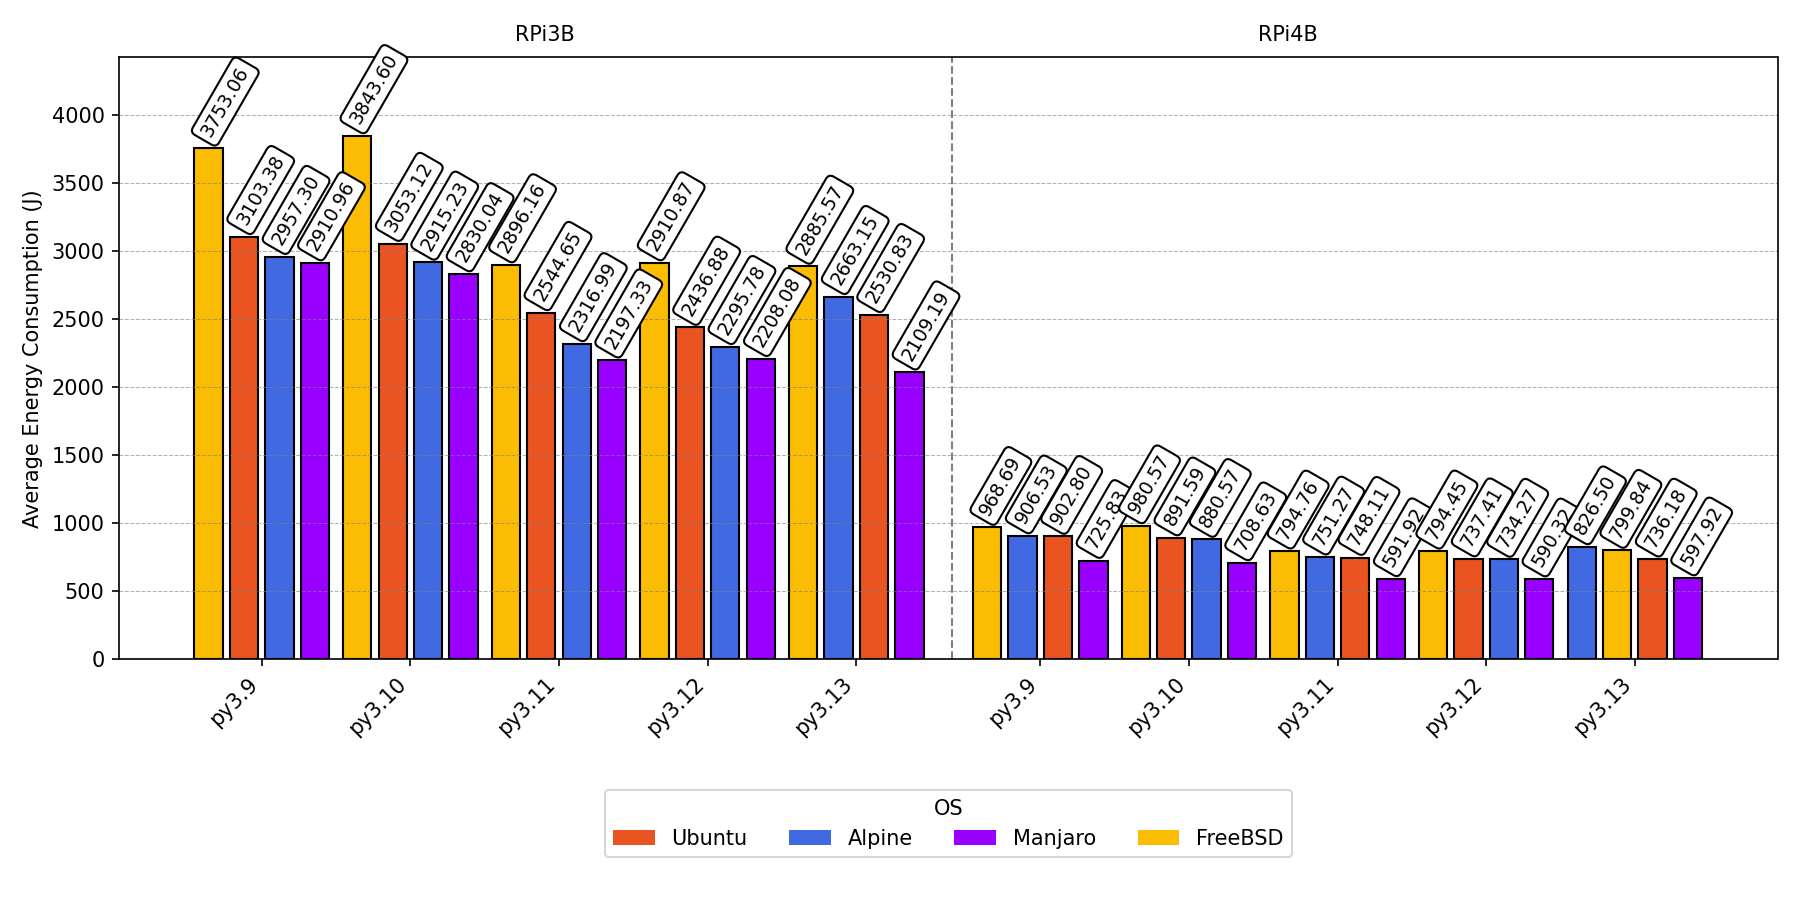
\includegraphics[width=\textwidth]{figures/consumption_barplot_all_pis.png}
    \caption{Barplot showing the average energy consumption across the 10 recordings made for each configuration.}
    \label{fig:barplot}
\end{figure}

\autoref{fig:barplot} shows the average energy consumption of all benchmarked configurations. The average energy consumption is reflected in both the height of the given column and the label displayed above it. OSs are displayed grouped by Python versions, ordered from lowest to highest version left to right. Within Python version groupings, the OSs are ordered from highest to lowest average energy consumption from left to right. This figure visually indicates, like observed above, RPi3B+ on FreeBSD running Python3.10 having the highest average energy consumption and RPi4B on Manjaro running Python3.12 having the lowest. The figure also clearly indicates a large difference in average energy consumption between the RPi3B+ and RPi4B. A hierarchy between OSs also presents itself, with FreeBSD consistently having the highest energy consumption within a given group (except for Python3.13 on the RPi4B) and Manjaro consistently having the lowest. The hierarchy between Python versions is less clear, but there does seem to be a trend of the higher version having the lower average energy consumption.

\begin{figure}[H]
    \centering
    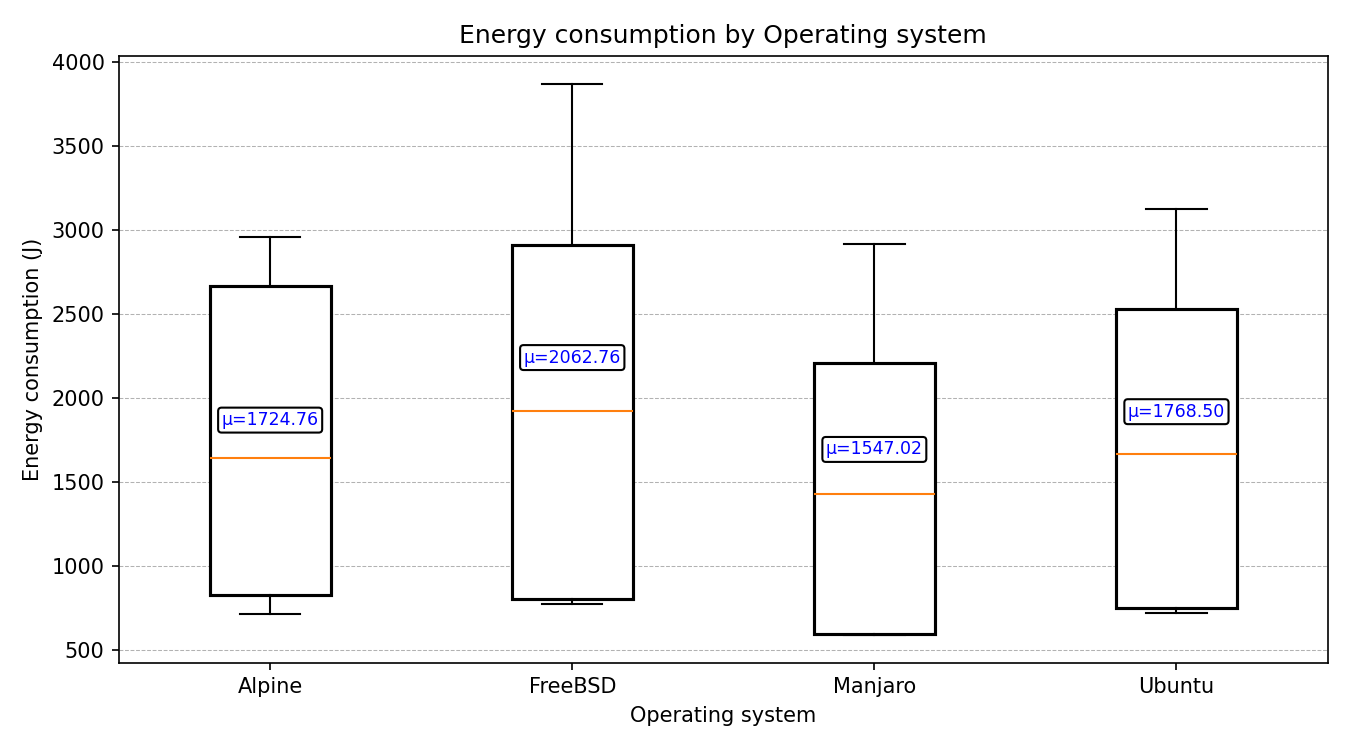
\includegraphics[width=\textwidth]{figures/energy_boxplot_by_os.png}
    \caption{Boxplot showing the energy consumption of operating systems across all hardware setups and Python versions.}
    \label{fig:boxplot_os}
\end{figure}

\autoref{fig:boxplot_os} shows the energy consumption statistics of OSs across all Python and RPi versions. The minimum is shown by the bottom black line under the white box, the 25th quartile by the bottom of the white box, the median by the orange line, the 75th quartile by the top of the white box, the maximum by the top black bar above the white box and the average ($\mu$) written in blue. These values are extracted from all recordings made for the given OS, such that each box therefore represents 100 individual recordings across 10 configurations. Here we see again a hierarchy of energy consumption, with FreeBSD being highest and Manjaro lowest. We also see an indication that outliers among groups are skewed towards high energy consumption, with the maximum being far removed from the 75th and 25th quartiles. This pattern also indicates that our data for OSs is not normally distributed, but skewed towards the lower end of energy consumption.

\begin{figure}[H]
    \centering
    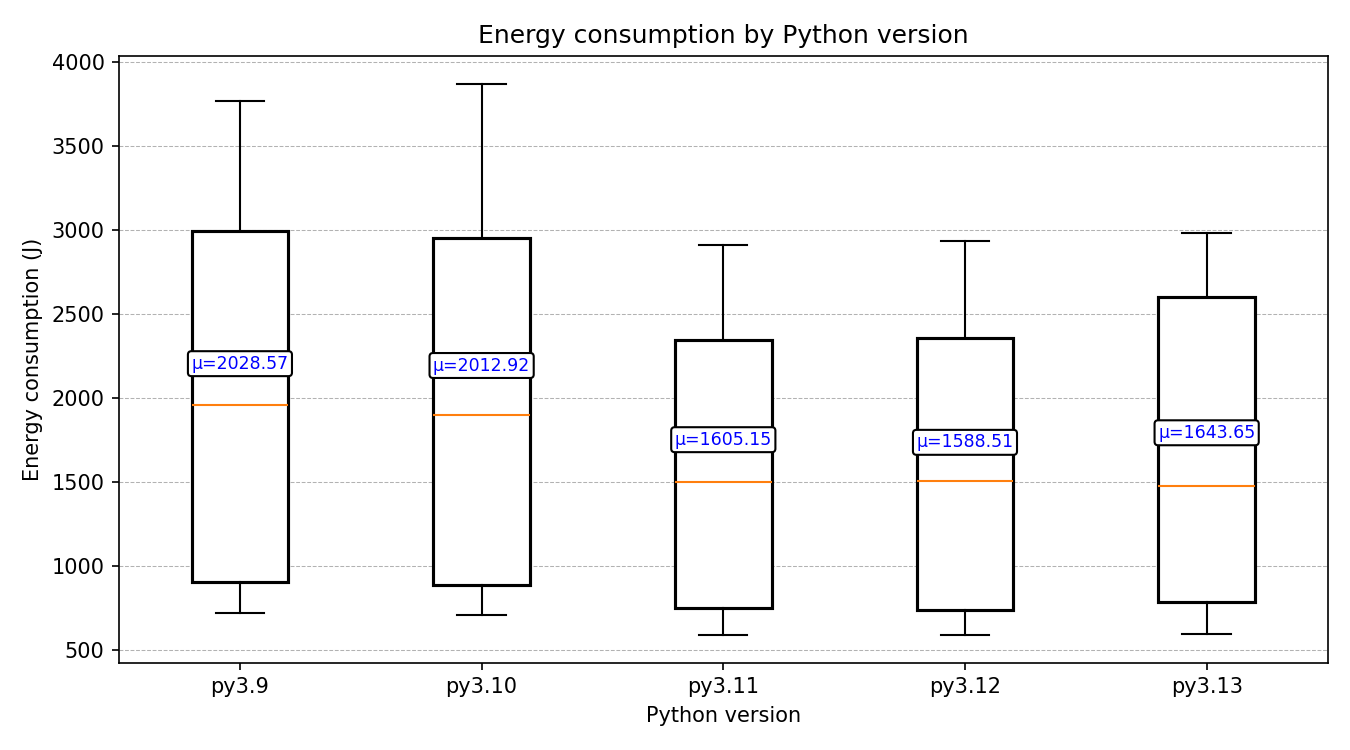
\includegraphics[width=\textwidth]{figures/energy_boxplot_by_python.png}
    \caption{Boxplot showing the energy consumption of Python versions across all hardware setups and operating systems.}
    \label{fig:boxplot_python}
\end{figure}

\autoref{fig:boxplot_python} shows the energy consumption statistics of Python versions across all operating systems and RPi versions in the same way \autoref{fig:boxplot_os} did for operating systems. These values are accordingly extracted from all recordings made for the Python version, such that each box represents 80 individual recordings across 8 configurations. The hierarchy between Python versions is less clear, but there seems to be a clear decrease in energy consumption from Python3.11 onwards. This data also seems to be skewed towards lower energy consumption, but not as heavily as for OSs. Interestingly, while the values for Python3.11 and 3.12 seem almost equal, the values for Python3.13 seem to be shifted slightly upward, indicating higher energy consumption relative to versions 3.11 and 3.12.

\begin{figure}[H]
    \centering
    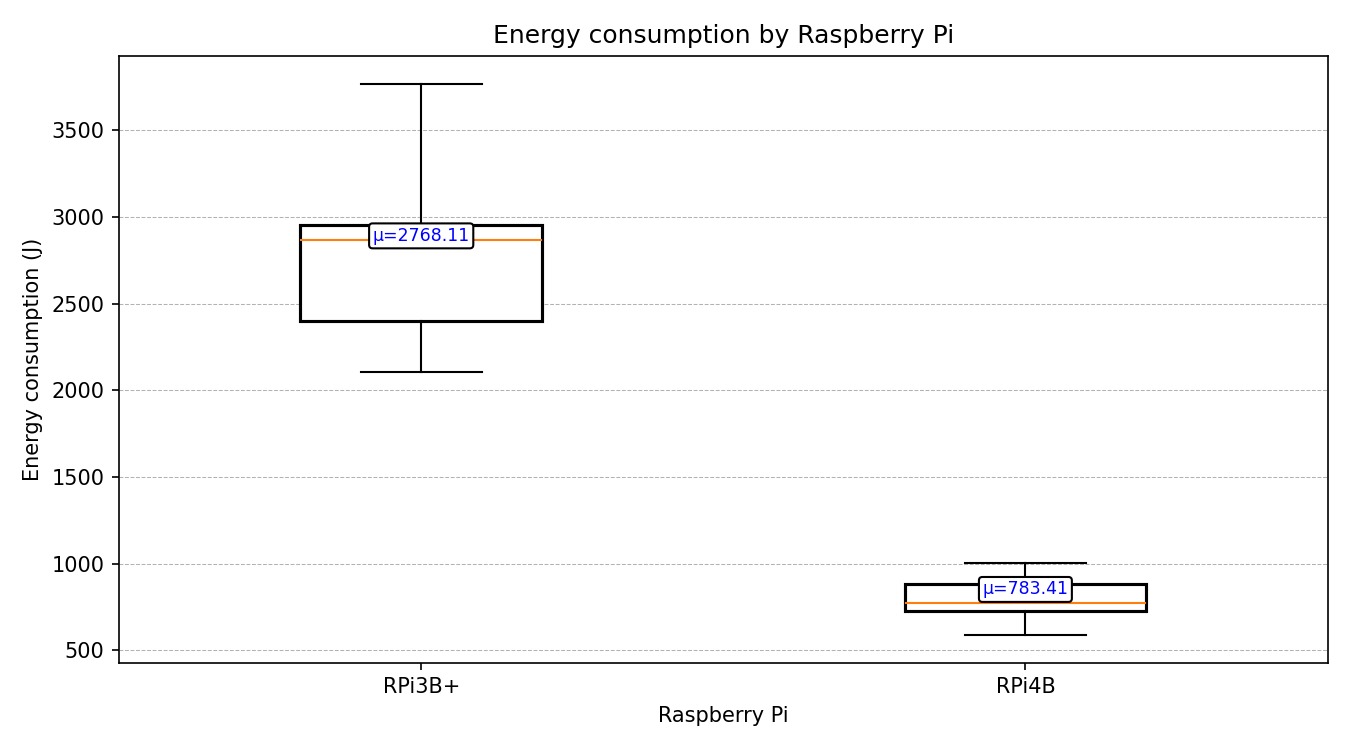
\includegraphics[width=\textwidth]{figures/energy_boxplot_by_rpi.png}
    \caption{Boxplot showing the energy consumption of RPi versions across all OSs and Python versions.}
    \label{fig:boxplot_rpi}
\end{figure}

\autoref{fig:boxplot_rpi} shows the same statistics as \autoref{fig:boxplot_os} and \autoref{fig:boxplot_python} for the two RPi versions. Each box therefore represents values extracted from 200 individual recordings across 20 configurations. The hierarchy between the two RPis here is readily apparent, with the RPi3B+ having higher energy consumption across the board. The RPi3B+ at first glance seems to have a much higher spread of values, but with recordings ranging from 2000J to well above 3500J compared to a range of just above 500J to around 1000J for the RPi4B, both RPis see just under a doubling in energy consumption from lowest to highest. Both RPis also display a quite balanced range, with only the RPi3B+ being slightly skewed towards lower energy consumption.
